%%%%%%%%%%%%%%%%%%%%%%%%%%%%%%%%%%%%%%%%%%%%%%%%%%%%%%%%%%%%%%%%%%%%%%%%%%%%%%%%%%%%%
%%%%%%%%%%%%%%%%%%%%%%%%%%%%%%%%%%%%%%%%%%%%%%%%%%%%%%%%%%%%%%%%%%%%%%%%%%%%%%%%%%%%%
%%%%%%%%%%%%%%%%%%%%%%%%%%%%%%%%%%%%%%%%%%%%%%%%%%%%%%%%%%%%%%%%%%%%%%%%%%%%%%%%%%%%%
%%%%%%%%%%%%%%%%%%%%%%%%%%% STAN POCZATKOWY PROJEKTU %%%%%%%%%%%%%%%%%%%%%%%%%%%%%%%%
%%%%%%%%%%%%%%%%%%%%%%%%%%%%%%%%%%%%%%%%%%%%%%%%%%%%%%%%%%%%%%%%%%%%%%%%%%%%%%%%%%%%%
%%%%%%%%%%%%%%%%%%%%%%%%%%%%%%%%%%%%%%%%%%%%%%%%%%%%%%%%%%%%%%%%%%%%%%%%%%%%%%%%%%%%%
%%%%%%%%%%%%%%%%%%%%%%%%%%%%%%%%%%%%%%%%%%%%%%%%%%%%%%%%%%%%%%%%%%%%%%%%%%%%%%%%%%%%%

\chapter{Stan początkowy projektu}
\label{cha:pocz}

\section{Architektura}

\section{Budowanie} 
Niniejsza część pracy zawiera opis pierwotnego sposobu budowania aplikacji, wraz z zastosowanymi rozwiązaniami technologicznymi (struktura i zawartość plików CMake) oraz listą potencjalnych ograniczeń wynikających z dotychczasowego podejścia do budowania.

\paragraph*{Struktura plików CMake}\mbox{}\\
% Opisac co gdzie jest, za co odpowiadają poszczegolne szablony
Projekt w swojej oryginalnej postaci budowany był za pomocą narzędzia CMake w wersji \textbf{2.8}. Wyróżnić można było jeden nadrzędny plik \textit{CMakeLists.txt} znajdujący się w katalogu głownym projektu oraz pomniejsze pliki dla każdego z modułów. Rysunek przedstawia w uproszczeniu pierwotną strukturę projektu, z wyszczególnieniem plików odpowiedzialnych za jego budowanie.

\textbf{TODO: tutaj dac jakis fajny rysuneczek}












\paragraph*{Obsługa bibliotek zewnętrznych}\mbox{}\\
% Opisac, jak obsługiwany jest Boost, GSL, Caen



\paragraph*{Ograniczenia pierwotnego systemu budowania}\mbox{}\\
% Cos jeszcze dopisac, zrobic zeby sie to lepiej czytalo
Pierwotna wersja projektu narzuca daleko idące ograniczenia na sposób jego budowania. Najważniejszym z nich jest brak bezpośredniej możliwości zbudowania pojedynczych komponentów projektu. Listing \ref{lst:orig} przedstawia fragment oryginalnego pliku \textit{CMakeLists.txt} znajdującego się w katalogu głównym projektu. \textbf{TUTAJ REF DO PRACY PLUTECKIEGO} Plik ten pozwala na zbudowanie trzech aplikacji wchodzących w skład oprogramowania projektu GGSS: \textit{ggssrunner}, \textit{dimCS} oraz opcjonalnie \textit{ggsspector}. Jest to jedyny plik w całym projekcie zawierający wszystkie informacje konieczne do zbudowania wymienionych aplikacji - tzn. posiadający listę bibliotek, od których aplikacje te są zależne. Oznacza to, że niemożliwe jest zbudowanie aplikacji \textit{ggssrunner} jedynie za pomocą dedykowanego jej pliku \textit{CMakeLists.txt}. Zatem pomimo, iż struktura projektu jest zmodularyzowana jeśli chodzi o architekturę (oprogramowanie zostało podzielone na biblioteki), to niemożliwe jest (w prosty sposób, za pomocą dostarczonych plików \textit{CMakeLists.txt}) zbudowanie pojedynczych modułów projektu.

\begin{lstlisting}[language=bash, caption={Fragment oryginalnego pliku CMakeLists.txt znajdującego się w katalogu głównym pierwotnej wersji projektu}, label={lst:orig}]
# array with used libraries
set(PROJECTS
        logLib
        xmlLib
        utilsLib
        handleLib
        ThreadLib
        fifoLib
        FitLib
        OrtecMcbLib
        CaenHVLib
        ggssLib
        usbrmLib
        CaenN1470Lib
        mcaLib
        daemonLib
        )

foreach (singleproject ${PROJECTS})
        parse_directory(${singleproject})
endforeach(singleproject)

# executables
add_subdirectory (_ggss) # ggssrunner binary
add_subdirectory (_dimCS) #dimCS binary
if(BUILD_GGSSPECTOR)
    add_subdirectory (_ggsspector) #ggsspector binary
endif()
\end{lstlisting}

Budowanie projektu za pomocą pliku, którego fragment przedstawia listing \ref{lst:orig} opiera się na liście zależności przechowywanej w zmiennej \textit{PROJECTS}. Umożliwia to stosunkowo łatwe rozszerzanie projektu o nowe biblioteki - wystarczy dopisać nazwę katalogu z biblioteką do listy zależności. Wadą tego rozwiązania jest natomiast brak możliwości wywnioskowania zależności zachodzących w projekcie. Listing \ref{lst:origggss} przedstawia plik \textit{CMakeLists.txt} służący do budowania aplikacji \textit{ggssrunner}. Na podstawie tych dwóch plików można jedynie wywnioskować, że aplikacja \textit{ggssrunner} jest zależna od wszystkich bibliotek, których nazwy znaleźć można w zmiennej \textit{PROJECTS}. Nie ma natomiast możliwości identyfikacji zależności między samymi bibliotekami. Takie podejście utrudnia zrozumienie struktury projektu, co bezpośrednio prowadzi do problemów z jego rozwojem.

%% Dodac bardziej szczegolowy opis tego projektu
\begin{lstlisting}[language=bash, caption={Oryginalny plik CMakeLists.txt służacy budowania aplikacji ggssrunner.}, label={lst:origggss}]
project (_ggss)
add_executable (ggssrunner main)
target_link_libraries (ggssrunner ${PROJECTS})
install(TARGETS ggssrunner RUNTIME DESTINATION bin)
\end{lstlisting}




\section{Dostarczanie i uruchamianie}

\section{Kontrola wersji}


%%%%%%%%%%%%%%%%%%%%%%%%%%%%%%%%%%%%%%%%%%%%%%%%%%%%%%%%%%%%%%%%%%%%%%%%%%%%%%%%%%%%%
%%%%%%%%%%%%%%%%%%%%%%%%%%%%%%%%%%%%%%%%%%%%%%%%%%%%%%%%%%%%%%%%%%%%%%%%%%%%%%%%%%%%%
%%%%%%%%%%%%%%%%%%%%%%%%%%%%%%%%%%%%%%%%%%%%%%%%%%%%%%%%%%%%%%%%%%%%%%%%%%%%%%%%%%%%%
%%%%%%%%%%%%%%%%%%%%%%%%%%% STAN DOCELOWY PROJEKTU %%%%%%%%%%%%%%%%%%%%%%%%%%%%%%%%%%
%%%%%%%%%%%%%%%%%%%%%%%%%%%%%%%%%%%%%%%%%%%%%%%%%%%%%%%%%%%%%%%%%%%%%%%%%%%%%%%%%%%%%
%%%%%%%%%%%%%%%%%%%%%%%%%%%%%%%%%%%%%%%%%%%%%%%%%%%%%%%%%%%%%%%%%%%%%%%%%%%%%%%%%%%%%
%%%%%%%%%%%%%%%%%%%%%%%%%%%%%%%%%%%%%%%%%%%%%%%%%%%%%%%%%%%%%%%%%%%%%%%%%%%%%%%%%%%%%

\chapter{Stan docelowy projektu}
\label{cha:docel}
Niniejszy rozdział zawiera opis docelowej wersji systemu GGSS, jaka powinna zostać osiągnięta po zakończeniu przez autorów prac. Cele do zrealizowania podzielone zostały na dwie główne części, wynikające z organizacji czasowej prac tzn. wkład autorów w system nie zamyka się wraz z zakończeniem prac nad niniejszym manuskryptem. Z tego powodu niniejszy rodział podzielony został na dwie części - pierwsza z nich opisuje finalną wersję projektu, natomiast druga - wersję po zakończeniu prac w ramach projektu inżynierkiego.

\section{Finalna wersja projektu}
Projekt w swojej wersji finalnej ma charakteryzować się modularną architekturą zarówno jeśli chodzi o organizację kodu, jak i sposób jego budowania. Pozwala to na proste i efektywne testowanie każdego komponentu z osobna. Ułatwia to również podmianę komponentów w środowisku produkcyjnym. Większa modularyzacja pozwala skrócić czas poszukiwania źródła ewentualnych błędów w działaniu systemu. Z drugiej natomiast strony podział systemu na dużą liczbę komponentów utrudnia proces budowania, przez co wymagana jest jego znacząca automatyzacja. Konieczne jest przygotowanie więc prostej w użytkowaniu infrastruktury wspomagającej proces produkcyjny. Powinna być ona dobrze udokumentowana, by próg wejścia do projektu był możliwie niski. Powinny więc zostać przygotowane instrukcje w języku angielskim zawierające zestaw najczęściej używanych komend wraz z wariantami ich użycia (np. flagi). Kluczowym celem jest również modernizacja kodu źródłowego - zarówno jeśli chodzi o jego jakość, jak i zastosowane technologie. Projekt charakteryzować się ma więc ustandaryzowanym, ogólnoprzyjętym przez społeczność programistów jako tzw. \textit{dobre praktyki}, nazewnictwem, odpowiednim podziałem na poziomie kodu źródłowego (funkcje, klasy itp.). W swojej ostatecznej wersji projekt powinien bazować na najnowszych, dostępnych w ramach infrastruktury produkcyjnej CERN-u, technologiach, np. standard języka C++. Dzięki temu zależności zewnętrzne powinny zostać ograniczone do minimum, na rzecz standardowych rozwiązań (np. biblioteka standardowa), by zagwarantować możliwie duża przenośność. Zaplanowano również rozszerzenie projektu o nowe komponenty ułatwiające korzystanie z systemu (np. graficzny interfejs użytkownika).

\section{Stan oczekiwany w ramach projektu inżynierskiego}
Z uwagi na brak możliwości realizowania wszystkich powyższych postulatów dotyczących celów pracy w ramach projektu inżynierkiego (co wynika z ograniczonego czasu), wybrany został następujący podzbiór wymagań:
\begin{itemize}
\item przygotowanie środowiska umożliwijącego zarządzanie prowadzonym projektem
\item modularyzacja projektu (z poziomu architektury i systemu budowania \textit{CMake})
\item przygotowanie infrastruktury automatyzującej proces produkcyjny, zapewniającej spójne środowisko do testowania
\item wykonanie dokumentacji zgodnej z wymienionymi założeniami
\item wprowadzenie standardu nazewnictwa na poziomie procesu budowania i podziału na repozytoria
\item przeprowadzenie testów wynikowego produktu
\end{itemize}
Rezultatem zakończenia tej części prac powinien być w pełni działający, udoskonalony system.


%%%%%%%%%%%%%%%%%%%%%%%%%%%%%%%%%%%%%%%%%%%%%%%%%%%%%%%%%%%%%%%%%%%%%%%%%%%%%%%%%%%%%
%%%%%%%%%%%%%%%%%%%%%%%%%%%%%%%%%%%%%%%%%%%%%%%%%%%%%%%%%%%%%%%%%%%%%%%%%%%%%%%%%%%%%
%%%%%%%%%%%%%%%%%%%%%%%%%%%%%%%%%%%%%%%%%%%%%%%%%%%%%%%%%%%%%%%%%%%%%%%%%%%%%%%%%%%%%
%%%%%%%%%%%%%%%%%%%%%%%%%%% OGRANICZENIA INFRASTRUKTURY %%%%%%%%%%%%%%%%%%%%%%%%%%%%%
%%%%%%%%%%%%%%%%%%%%%%%%%%%%%%%%%%%%%%%%%%%%%%%%%%%%%%%%%%%%%%%%%%%%%%%%%%%%%%%%%%%%%
%%%%%%%%%%%%%%%%%%%%%%%%%%%%%%%%%%%%%%%%%%%%%%%%%%%%%%%%%%%%%%%%%%%%%%%%%%%%%%%%%%%%%
%%%%%%%%%%%%%%%%%%%%%%%%%%%%%%%%%%%%%%%%%%%%%%%%%%%%%%%%%%%%%%%%%%%%%%%%%%%%%%%%%%%%%

\chapter{Ograniczenia dostępnej infrastruktury}
\label{cha:ogra}
Z uwagi na silny związek oprogramowania GGSS z infrastrukturą CERN oraz wymóg zapewnienia możliwości budowania projektu na należących do niej maszynach, przed autorami postawiony został szereg ograniczeń związanych z możliwymi do użycia technologiami oraz sposobem wykonywania pewnych operacji. Niniejszy rozdział stanowi opis najważniejszych z tych ograniczeń z uwzględnieniem ich wpływu na obraną przez autorów pracy ścieżkę rozwoju projektu.


\section{Ograniczone uprawnienia w środowisku docelowym}


\section{Wersje kompilatorów i interpreterów}
Dostępne wersje kompilatorów i interpreterów stanowią jeden z kluczowych czynników, który należy uwzględnić podczas wprowadzania zmian w istniejącym systemie, ponieważ definiują one możliwy do wykorzystania podzbiór technologii. W kontekście systemu GGSS ograniczenia te dotyczą przede wszystkim kompilatora języka C++ oraz interpretera języka Python. 

\paragraph*{Wersja kompilatora języka C++}\mbox{}\\
Dostępna w ramach infrastruktury projektu wersja kompilatora języka C++ to \textbf{g++ (GCC) 4.8.5}. Wspiera ona w pełni standard C++11, czyli funkcjonalności takie, jak referencje do r-wartości, wyrażenia lambda czy zakresowa pętla for \cite{GCC48}. Wersja ta nie wspiera niestety nowszych wydań języka (C++14/17).

\paragraph*{Wersja interpretera języka Python}\mbox{}\\
Domyślną wersją Pythona jest \textbf{Python 2.7.5}, jednak dostępny jest również Python 3 (w wersji \textbf{Python 3.6.8}). Z uwagi na wspomniany wcześniej koniec oficjalnego wsparcia dla Pythona 2, który ma nadejść wraz z początkiem 2020 roku, naturalnym jest więc wybór wersji 3. Infrastruktura projektu posiada jednak znaczące braki jeśli chodzi o dostępne dla wersji 3 biblioteki zewnętrzne - domyślnie nie jest np. dostępna biblioteka \textit{Beautiful Soup}, slużąca do przetwarzania dokumentów w formacie HTML. Niektóre popularne bibliteki i frameworki (np. \textit{PyTest} - wykorzystywany do przeprowadzania testów oprogramowania) nie są dostępne dla obu wersji Pythona. Taka sytuacja wymusza więc wykorzystanie narzędzia \textit{virtualenv} w celu ich instalacji w odizolowanym środowisku, nie mającym wpływu na infrastrukturę CERN-u.

\section{Wersja narzędzia budującego CMake}
Dostępna wersja narzędzia CMake stanowiła zdaniem autorów największe ograniczenie w czasie prac nad projektem. Na maszynach docelowych dostępna jest jedynie stara wersja \textbf{2.8.12.2}. Nowsza wersja (\textbf{3.14.6}) dostępna jest na niektórych z komputerów, jednak z uwagi na konieczność zachowania kompatybilności ze wspomnianymi maszynami docelowymi, nie było możliwe jej użycie. Stosowanie wersji o numerze niższym od \textbf{3.0} skutkuje szeregiem ograniczeń - brakuje w niej wielu funkcjonalności pozwalających na stosowanie ogólnoprzyjętych dziś praktyk, jak np. określenie zakresu wersji narzedzia CMake, w którym powinna mieścić się używana wersja, by projekt można było bez problemu zbudować, czy wsparcie dla instrukcji \textit{target\_link\_directories} \cite{NewInCMake}.

\section{Związek projektu z wersją jądra systemu}


%%%%%%%%%%%%%%%%%%%%%%%%%%%%%%%%%%%%%%%%%%%%%%%%%%%%%%%%%%%%%%%%%%%%%%%%%%%%%%%%%%%%%
%%%%%%%%%%%%%%%%%%%%%%%%%%%%%%%%%%%%%%%%%%%%%%%%%%%%%%%%%%%%%%%%%%%%%%%%%%%%%%%%%%%%%
%%%%%%%%%%%%%%%%%%%%%%%%%%%%%%%%%%%%%%%%%%%%%%%%%%%%%%%%%%%%%%%%%%%%%%%%%%%%%%%%%%%%%
%%%%%%%%%%%%%%%%%%%%%%%%%%% WYKONANE PRACE %%%%%%%%%%%%%%%%%%%%%%%%%%%%%%%%%%%%%%%%%%
%%%%%%%%%%%%%%%%%%%%%%%%%%%%%%%%%%%%%%%%%%%%%%%%%%%%%%%%%%%%%%%%%%%%%%%%%%%%%%%%%%%%%
%%%%%%%%%%%%%%%%%%%%%%%%%%%%%%%%%%%%%%%%%%%%%%%%%%%%%%%%%%%%%%%%%%%%%%%%%%%%%%%%%%%%%
%%%%%%%%%%%%%%%%%%%%%%%%%%%%%%%%%%%%%%%%%%%%%%%%%%%%%%%%%%%%%%%%%%%%%%%%%%%%%%%%%%%%%

\chapter{Wykonane prace}
\label{cha:prace}

\section{Wykorzystanie funkcjonalności portalu Gitlab wspierających zarządzanie projektem}

\newpage
\section{Migracja projektu do systemu kontroli wersji Git i zmiany w architekturze}



\section{Zmiana sposobu budowania aplikacji} \label{buildingNew}
% Zarys rozwiazania
% Szablony + Boost + GSL
% Budowanie bibliotek
% Budowanie aplikacji
% DIM - skrypt do pobierania, budowanie jak external_project
% Skrypty do budowania calosci (+ sposoby budowania) + glowny CMake

\newpage
\section{Zastosowanie podejścia CI/CD}
Ważną częścia wykonanych prac było przygotowanie środowiska pozwalającego na zautomatyzowane budowanie i dystrybucję aplikacji. Standardowym dziś sposobem na rozwiązanie tego problemu jest podejście \textbf{CI/CD}. Skrót CI oznacza tzw. \textbf{ciągłą integrację} (\textit{Continous Integration}) - praktykę polegającą na stosowaniu współdzielonego repozytorium kodu źródłowego, za pomocą którego programiści pracujący nad projektem regularnie integrują swoje zmiany. Nowa wersja kodu jest automatycznie sprawdzana - serwer ciągłej integracji samodzielnie buduje projekt i uruchamia przygotowane dla niego testy. Skrót CD oznacza natomiast \textbf{ciągłe dostarczanie} (\textit{Continous Delivery}). Polega ono na przygotowaniu produktu do stanu, w którym jest on możliwy do wdrożenia w środowisku produkcyjnym. Może to być np. przeprowadzenie różnego rodzaju testów czy przygotowanie odpowiedniej paczki z aplikacją. Ważne jest, że w podejściu tym nie następuje automatyczne wdrożenie aplikacji do środowiska produkcyjnego (jest to domena \textbf{ciągłego wdrażania} \cite{CICDDef}, które jednak nie znalazło zastosowania w projekcie GGSS). Podejście \textbf{CI/CD} porównuje się czasem do działania linii produkcyjnej. Rysunek \ref{fig:cicd} obrazuje schematycznie jego działanie. 

\begin{figure}[H]
\centering
\caption{Przykładowy schemat działana podejścia \textit{Continous Integration / Continous Delivery}. Należy zwrócić uwagę, że w zastosowaniu praktycznym kolejność oraz liczba etapów może być różna od widocznej}
\label{fig:cicd}
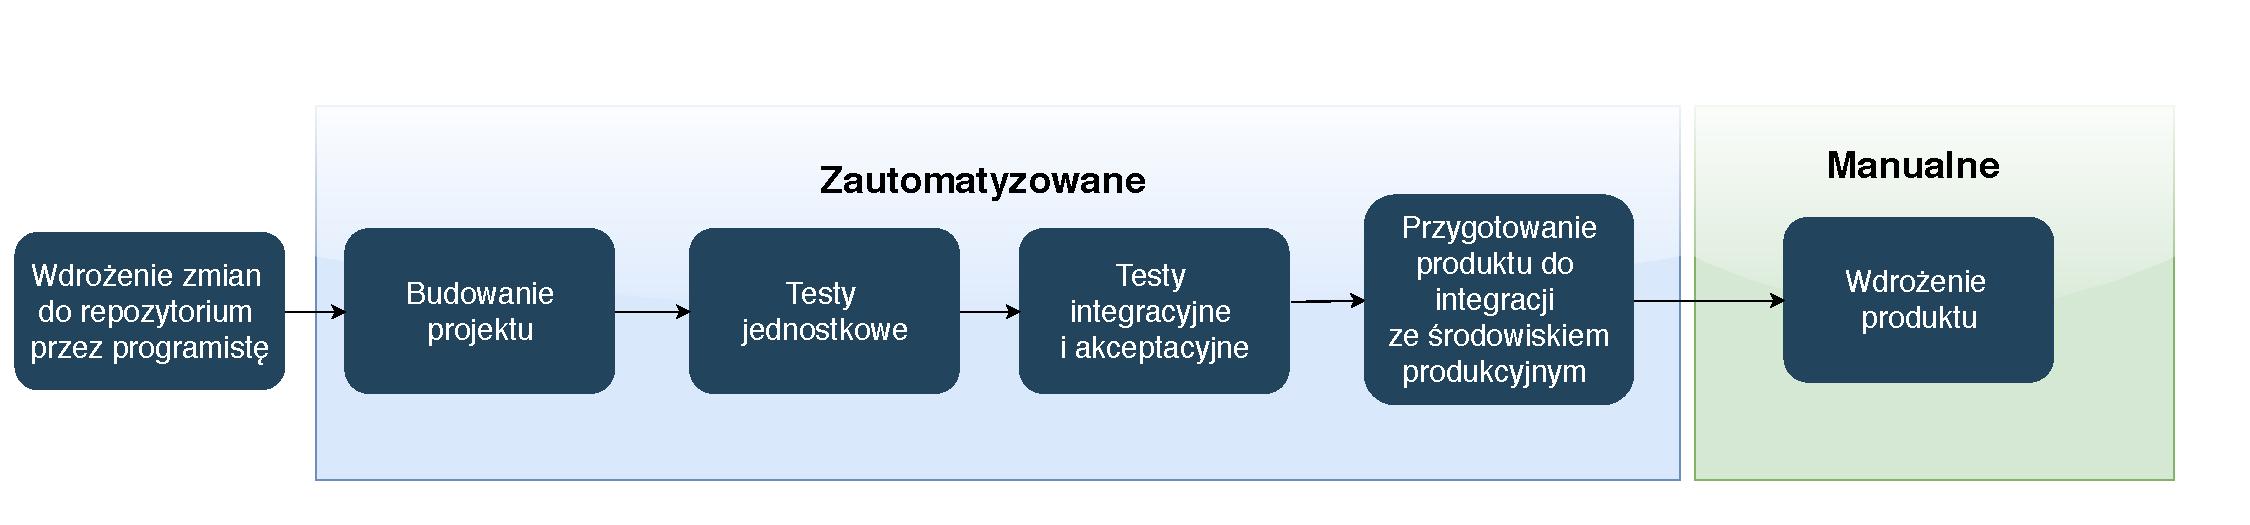
\includegraphics[width=\textwidth]{res/CICD.pdf}
\end{figure}

W kontekście systemu GGSS podejście to jest pożądane, z uwagi na konieczność zachowania poprawności działania systemu pomimo zmian (które aktualnie mają miejsce) w strukturze jego oprogramowania. Głównym celem jego zastosowania było ułatwienie autorom pracy działania jako zespół. Miało również znacząco przyspieszyć proces testowania aplikacji w środowisku produkcyjnym poprzez automatyczne tworzenie paczki z odpowiednią wersją oprogramowania.

\subsection{Możliwe sposoby implementacji podejścia CI/CD w projekcie GGSS}
Istnieje wiele narzędzi pozwalających na implementację ciągłej integracji oraz ciągłego dostarczania w projekcie. Prawodopodobnie najpopularniejszym z nich jest \textbf{Jenkins}. Jest to darmowe \cite{JenkinsWiki} oprogramowanie do automatyzacji, charakteryzujące się dużą konfigurowalnością. Przez lata stał się standardem dla wielu firm wytwarzających oprogramowanie. Jednak jego główną wadą, wykluczającą jego użycie w projekcie GGSS, jest zbyt duża ilość pracy związanej z jego konfiguracją i utrzymaniem. Narzędzie to sprawdza się dobrze przy dużej wielkości projektach. W przypadku systemu GGSS użytkowanie go przyniosłoby więcej pracy niż dałoby realnych korzyści. 

Autorzy zdecydowali się więc wykorzystać narzędzie CI/CD udostępniane przez portal \textbf{GitLab}. GitLab CI/CD udostępnia wystarczająco dużo możliwości, by możliwe było wprowadzenie automatyzacji budowania i testowania w systemie GGSS. Narzędzie to można wykorzystać na dwa sposoby:
\begin{itemize}
\item implementując mechanizm budowania i testowania manualnie, co daje większą kontrolę nad całym procesem
\item używając narzędzia \textbf{Auto DevOps}, oferującego predefiniowane konfiguracje ciągłej integracji i ciągłego dostarczania
\end{itemize}
Początkowo podjęta została decyzja o zastosowania drugiego z wyżej wymienionych rozwiązań. Przemawiającym za tym argumentem było potencjalne uproszczenie procedury wdrażania podejścia CI/CD do projektu - w portalu GitLab włączenie narzędzia Auto DevOps sprowadza się do zaznaczenia jednej opcji w ustawieniach na poziomie grupy lub repozytorium. Oferuje ono funkcjonalności takie, jak automatyzacja budowania i testowania projektu czy testy jakości kodu \cite{AutoDevOpsPage}. Podczas prób integracji tego rozwiązania do projektu pojawiło się jednak wiele problemów natury technicznej, związanych m.in. z niestandardowym sposobem działania projektu GGSS czy infrastrukturą tzw. \textit{runner-ów} używaną w CERN. Ostatecznie pomysł ten został więc porzucony na rzecz manualnej konfiguracji środowiska CI/CD. 

\subsection{Opis działania GitLab CI/CD}
Przed przystąpieniem do opisu sposobu zastosowania narzędzia GitLab CI/CD w projekcie GGSS przedstawiony zostanie sposób jego działania oraz najważniejsze pojęcia z nim zmiązane. Manualna konfiguracja polega na umieszczeniu w repozytorium pliku \textit{.gitlab-ci.yml} zawierającego szczegółowy opis przebiegu całego procesu ciągłej integracji i dostarczania (w tym konieczne do wykonania komendy). Przebieg ten określa się słowem \textbf{pipeline}. Składa się on z etapów (\textit{stages}), przy czym każdy etap może zawierać w sobie kilka równoległych zadań (\textit{jobs}). Idea ta została zilustrowana na Rys. \ref{fig:pipeline}.

\begin{figure}
\centering
\caption{Idea działania \textit{pipeline}. Kolorem czerwonym oznaczone zostały poszczególne etapy (\textit{stages}), natomiast zadania (\textit{jobs}) przedstawione zostały za pomocą ciemnoniebieskich prostokątów. Rysunek przedstawia przykładową strukturę, liczba etapów i zadań różni sie zwykle od pokazanej.}
\label{fig:pipeline}
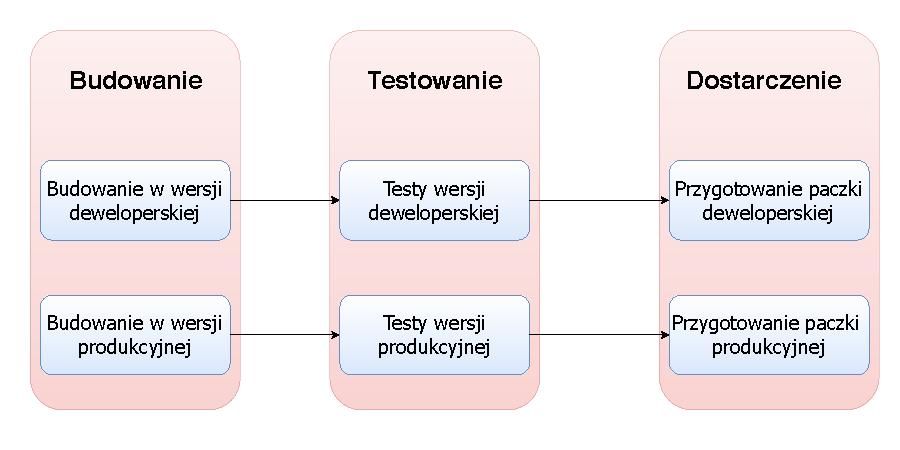
\includegraphics[width=\textwidth]{res/Pipeline.pdf}
\end{figure}

Wynikiem każdego z zadań może być tzw. \textbf{artefakt}, czyli możliwe do pobrania archiwum zawierające np. plik wykonywalny z produktem. Artefakty mogą być również przekazywane między poszczególnymi etapami procesu. 

Zadania składające się na pipeline uruchamiane są przez specjalne narzędzie \textbf{GitLab Runner}. Może on znajdować się na serwerach GitLab lub na skonfigurowanej przez klienta maszynie \cite{CIzGitLab}. Przebieg całego procesu koordynowany jest przez \textbf{GitLab Server} \cite{GitLabPage}.

Jak zostało wspomniane przebieg procesu CI/CD konfigurowany jest za pomocą specjalnego pliku \textit{.gitlab-ci.yml}. Zastosowany format \textit{YAML} (skrót od \textit{YAML Ain't Markup Language} \cite{YAMLWiki}), ze względu na swoją czytelność, pozwala na stosunkowo szybkie przygotowanie funkcjonalnego systemu. Listing \ref{lst:yml1} przedstawia przykład prostego pliku w tym formacie konfigurującego GitLab CI/CD. Na początku zostaje w nim określony użyty obraz \textit{Docker'a}, następnie wymienione są poszczególne etapy (klucz \textit{stages} - w tym przypadku jeden etap: \textit{software\_test}) procesu CI/CD, a na końcu pojawia sie opis zadania (\textit{dim\_software\_test}) należącego do zdefiniowanego etapu. Podczas definicji zadań możliwe jest wyspecyfikowanie mających się wykonać komend (klucz \textit{script}).

\begin{lstlisting}[caption={Przykład prostego pliku \textit{.gitlab-ci.yml} generującego jeden etap procesu CI/CD oraz jedno zadanie w ramach tego etapu}, label={lst:yml1}]
image: gitlab-registry.cern.ch/atlas-trt-dcs-ggss/ggss-misc/centos7

stages:
  - software_test

dim_software_test:
  stage: software_test
  script:
    - echo "Test"

\end{lstlisting}

\subsection{Opis automatyzacji za pomocą GitLab CI/CD w projekcie GGSS}
Na potrzeby projektu GGSS przygotowane zostało środowisko zapewniające ciągłą integrację i dostarczanie. Pozwala ono na automatyzację procesu budowania i testowania poszczególnych komponentów projektu oraz, dzięki mechanizmowi artekfaktów, przygotowuje gotowe paczki z najważniejszymi aplikacjami w projekcie (m.in. \textit{ggssrunner}). Każde repozytorium zawierające kompilowalny komponent projektu zostało wyposażone w plik \textit{.gitlab-ci.yml} konfigurujący zautomatyzowany proces budowania i testowania. W niniejszej części pracy zostaną przedstawione konfiguracje zrealizowane w ramach dwóch repozytoriów: \textit{ggss-all} oraz \textit{external-dim-lib}. 

W ramach repozytorium \textit{ggss-all} przygotowana została konfiguracja budująca aplikacje: \textit{ggss-runner}, \textit{ggss-dim-cs} oraz \textit{mca-n957}. Listing \ref{lst:ggssyml1} przedstawia fragment przygotowanego pliku \textit{.yml}. Plik ten zawiera siedem zadań zdefiniowanych w ramach etapu \textit{build} (nie ma konieczności bezpośredniej jego definicji, jest to jeden z trzech, obok \textit{test} i \textit{deploy}, etapów które mogą zostać, w razie pojawienia się przypisanego do nich zadania, wygenerowane automatycznie). Zadania te odpowiadają za:
\begin{itemize}
\item \textbf{build\_all\_debug\_static\_boost} - zbudowanie wszystkich trzech wymienionych wyżej aplikacji w wersji deweloperskiej (debug) ze statycznie dołączaną biblioteką Boost oraz przygotowanie artefaktu zawierającego wynikowe pliki wykonywalne.
\item \textbf{build\_all\_debug\_dynamic\_boost} - zbudowanie wszystkich trzech aplikacji w wersji deweloperskiej z dynamicznie dołączaną biblioteką Boost oraz przygotowanie artefaktu zawierającego wynikowe pliki wykonywalne.
\item \textbf{build\_all\_release\_static\_boost} oraz \textbf{build\_all\_release\_dynamic\_boost} - analogicznie do dwóch powyższych ale w wersji produkcyjnej (release).
\item \textbf{build\_only\_ggss\_runner}, \textbf{build\_only\_ggss\_dim\_cs} i \textbf{build\_only\_mca\_n957} - zbudowanie każdej aplikacji z osobna, bez produkowania artefaktu, w wersji debug z dynamicznie linkowaną biblioteką Boost (konfiguracja domyślna).
\end{itemize}

\begin{lstlisting}[caption={Fragment pliku \textit{.gitlab-ci.yml} konfigurującego \textit{pipeline} CI/CD dla repozytorium \textit{ggss-all}}, label={lst:ggssyml1}]
image: gitlab-registry.cern.ch/atlas-trt-dcs-ggss/ggss-misc/centos7

before_script:
  - git submodule update --init --remote --recursive

# Debug builds 

build_all_debug_static_boost:
  stage: build
  script:
    - mkdir build
    - cd build
    - python ../build.py -s --debug
  artifacts:
    name: all_debug_static_boost
    paths:
       - build/ggss-dim-cs-build/ggss-dim-cs
       - build/ggss-runner-build/ggss-runner
       - build/mca-n957-build/mca-n957

# Dalsza część pliku ...

\end{lstlisting}

Generowane w repozytorium \textit{ggss-all} artefakty są tymi trafiającymi ostatecznie do środowiska produkcyjnego. Pliki mające trafić do artefaktu specyfikowane są za pomocą klucza \textit{paths} (widoczne na listingu \ref{lst:ggssyml1}). Do przeprowadzenia budowania używany jest specjalnie w tym celu przygotowany przez autorów obraz, oparty na oficjalnych obrazach dostarczonych przez CERN. Rys. \ref{fig:pipelineall} przedstawia wynikowy \textit{pipeline} oraz dostępnie do pobrania artefakty.

\begin{figure}[H]
\centering

\begin{subfigure}{0.4\textwidth}
\centering
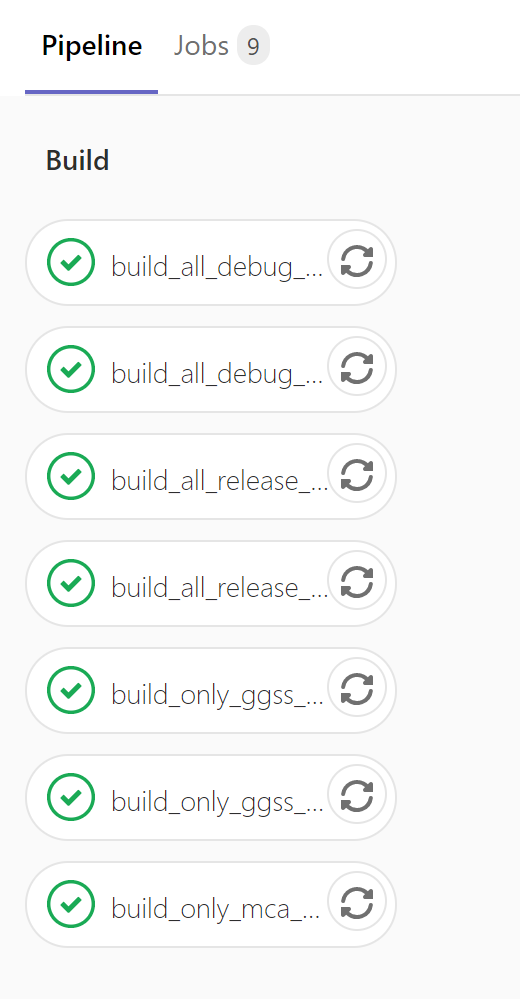
\includegraphics[height=9cm]{res/png/runnerPipeline}
\caption{\textit{Pipeline} wygenerowany na podstawie konfiguracji zamieszczonej w pliku \textit{.yml} (listing \ref{lst:ggssyml1})}
\end{subfigure}
\hspace{0.5cm}
\begin{subfigure}{0.4\textwidth}
\centering
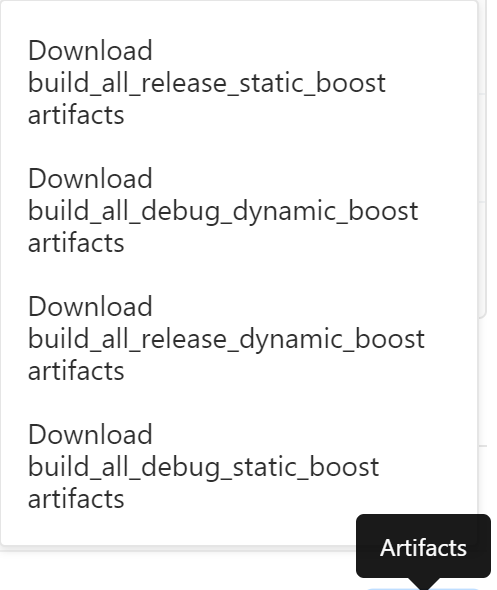
\includegraphics[height=9cm]{res/png/runnerArtifacts}
\caption{Możliwe do pobrania artefakty}
\end{subfigure}

\caption{Zrzuty ekranu wykonane w serwisie GitLab przedstawiające elementy działania ciągłej integracji i dostarczania dla repozytorium \textit{ggss-all}}
\label{fig:pipelineall}

\end{figure}

Konfiguracja stworzona na potrzeby repozytorium \textit{external-dim-lib} różni się nieznacznie od opisanej do tej pory jeśli chodzi o techniczną stronę jej realizacji. Przygotowany \textit{pipeline} (Rys. \ref{fig:pipelineDIM}) składa się z innych etapów i zadań, ale zostały one skonfigurowane z użyciem zaprezentowanych już technik. Na potrzeby przugotowania biblioteki obsługującej protokół \textit{DIM} zostały więc stworzone dwa etapy: odpowiadający za przeprowadzenie testów skryptu pobierającego bibliotekę ze strony internetowej (\textit{Software\_test}), oraz odpowiadający na zbudowanie jej w dwóch wersjach (\textit{Build}). Obie wersje udostępniane są do pobrania za pomocą mechanizmu artefaktów.  

\begin{figure}[H]
\centering
\caption{\textit{Pipeline} wygenerowany na potrzeby repozytorium \textit{external-dim-lib}}
\label{fig:pipelineDIM}
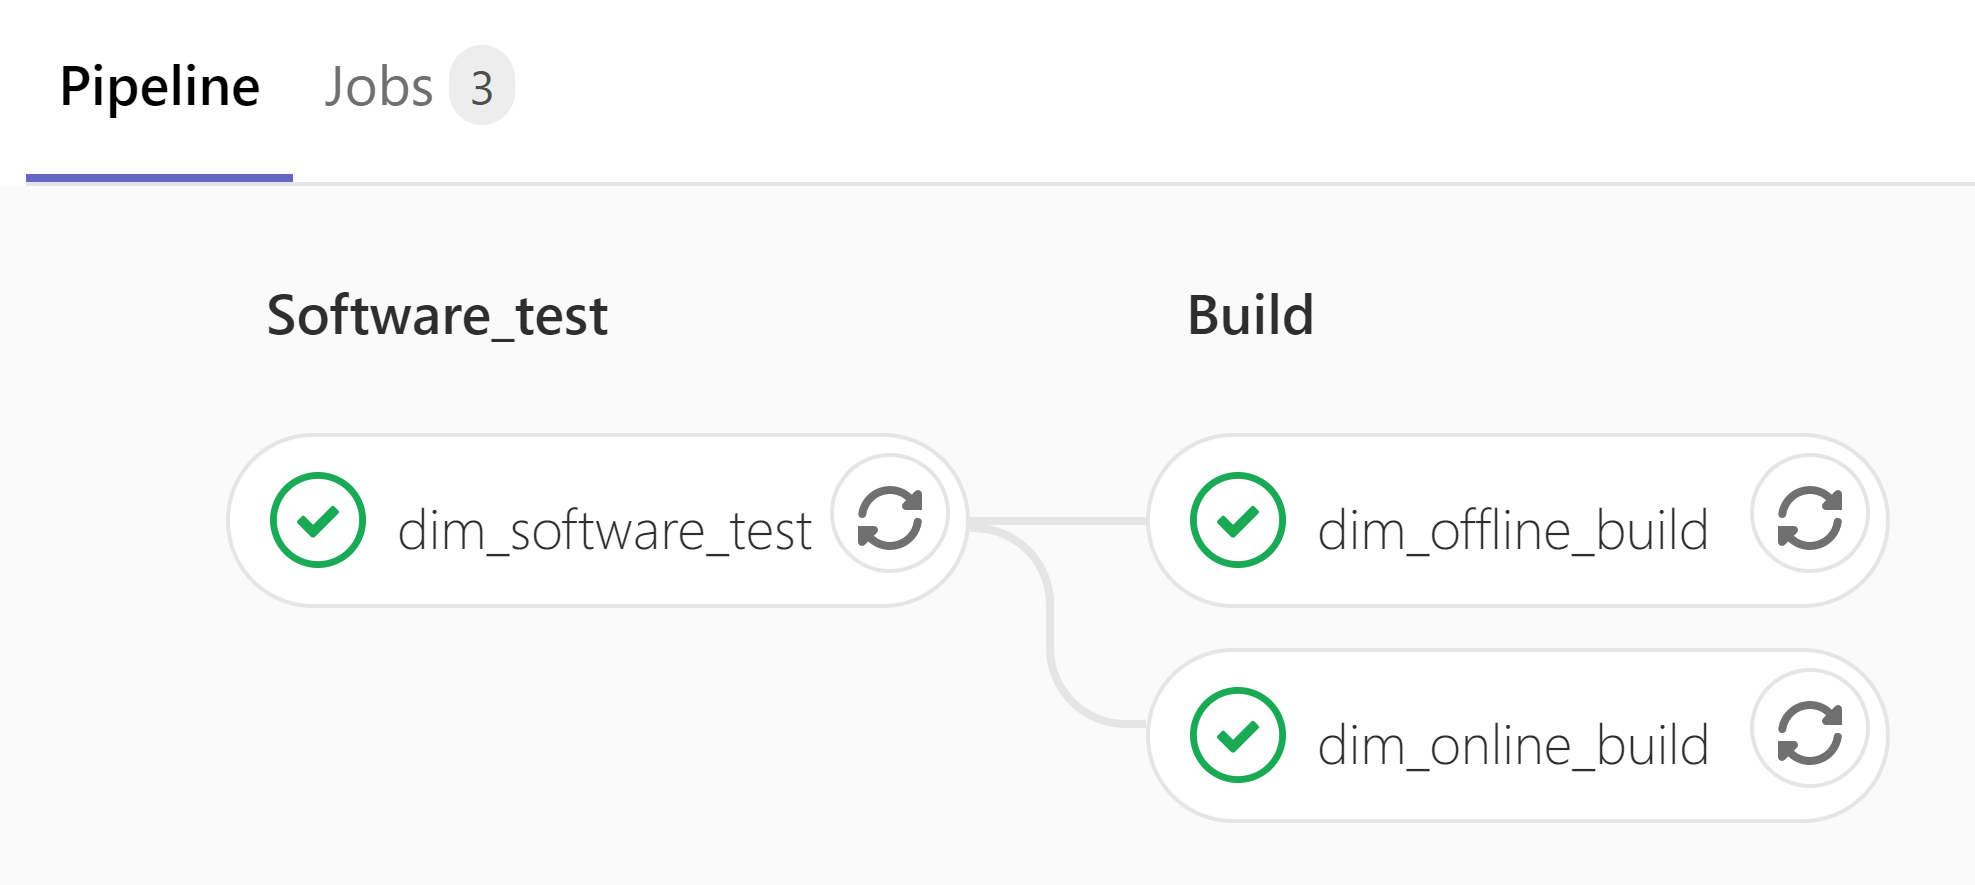
\includegraphics[width=\textwidth]{res/png/pipelineDIM}
\end{figure}

Podobnego typu prace zostały wykonane dla większości pozostałych repozytoriów. Z uwagi na ich powtarzalny charakter nie zostaną one jednak omówione w niniejszym manuskrypcie. 

W przedstawionym przykładzie dotyczącym aplikacji \textit{ggssrunner} (listing \ref{lst:ggssyml1}) znajduje się klucz \textit{before\_script} z instrukcją pobierającą submoduły projektu. Istnieją dwa wykluczające się sposoby na wykonanie tej czynności. Submoduł może zostać pobrany w swojej najnowszej wersji znajdującej się na \textbf{zdalnej rewizji} (tak jak w przytoczonym przykładzie, służy temu opcja \textbf{--remote}) lub w wersji \textbf{aktualnie powiązanej z repozytorium nadrzędnym} (realizację przedstawia listing \ref{lst:ggsscicdsoft}). Oba wymienione podejścia mają swoje wady i zalety. Rys. \ref{fig:submoduleProblem} stanowi uproszczoną (ograniczoną tylko do jednej gałęzi na repozytorium) ilustrację opisywanego problemu. Pierwszy z wymienionych sposobów jest wygodniejszy, ponieważ pozwala na dostarczenie i przetestowanie najnowszej możliwej wersji produktu. Jest to jednak ryzykowne - najnowsza wersja submodułu może nie być kompatybilna z modułem nadrzędnym (np. mógł zmienić się jej interfejs). Spowoduje to błąd, którego źródło może być trudne do odnalezienia (jeśli programista owej najnowszej wersji nie używał pojawi się sprzeczność w wynikach otrzymywanych przez niego lokalnie, a generowanych przez mechanizm CI/CD). Drugie rozwiązanie jest zatem bezpieczniejsze i gwarantuje stabilność. Autorzy skłaniają się w większości przypadków do tego własnie rozwiązania, jednak z uwagi na zalety pierwszej z wymienionych opcji, jest ona wciąż używana w niektórych repozytoriach (np. \textit{ggss-all}). 

\begin{lstlisting}[caption={Fragment pliku \textit{.gitlab-ci.yml} znajdującego się w repozytorium \textit{ggss-software-libs} pobierający submoduły projektu w wersji aktualnie powiązanej z repozytorium narzędnym}, label={lst:ggsscicdsoft}]
image: gitlab-registry.cern.ch/atlas-trt-dcs-ggss/ggss-misc/centos7

variables:
  GIT_SUBMODULE_STRATEGY: recursive

# Dalsza część pliku

\end{lstlisting}

\begin{figure}[H]
\centering
\caption{Uproszczona (ograniczona do jednej gałęzi na repozytorium) ilustracja problemu dotyczacego pobieranej przez mechanizm CI/CD wersji submodułu. Problem polega na podjęciu decyzji, czy powinna zostać pobrana wersja najnowsza (tutaj oznaczona jako \textit{commit\_D}) czy ta aktualnie powiązana z repozytorium nadrzędnym (\textit{commit\_B})}
\label{fig:submoduleProblem}
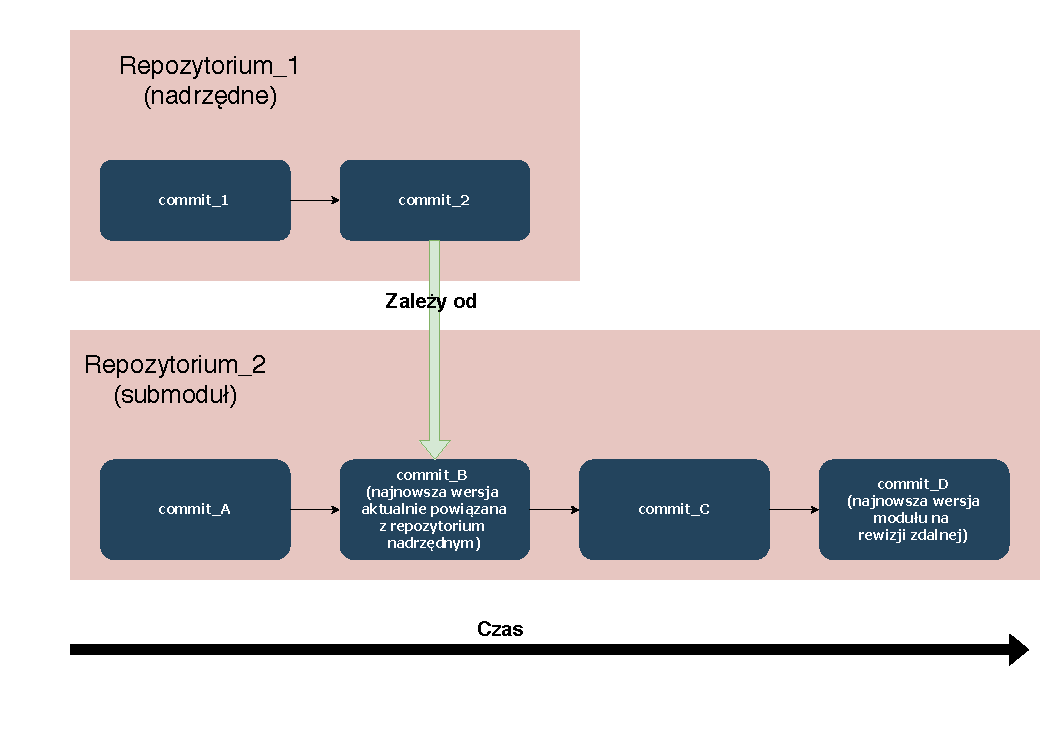
\includegraphics[width=\textwidth]{res/SubmodulesProblem}
\end{figure}


W ramach prac nad mechanizmem CI/CD w projekcie GGSS został również przygotowany specjalny \textbf{szablon} ułatwiający tworzenie \textit{pipeline'ów}. Został on umieszczony w repozytorium \textit{aux}, a jego fragment przedstawia listing \ref{lst:ggsscicdtempl}. Zawartość tego szablonu, zmodyfikowana zgodnie ze specyfiką danego repozytorium, posłużyła autorom do napisania większości plików \textit{.yml}, które znalazły się w projekcie.

\begin{lstlisting}[caption={Fragment szablonu ułatwiającego pisanie plików \textit{.gitlab-ci.yml} znajdującego się w repozytorium \textit{aux}}, label={lst:ggsscicdtempl}]
# This is gitlab-ci.yml for TRT GGSS project.

# actual image being used by ggss project
image: gitlab-registry.cern.ch/atlas-trt-dcs-ggss/ggss-misc/centos7

# variable needed for submodule clone - can be moved to job locally
# to use submodules on docker without adding ssh key please use relative submodules path
variables:
  GIT_SUBMODULE_STRATEGY: recursive

build:
  stage: build
# input your building under scripts
  script:
#    e.g:
#   - cmake
#   - make

#   artifacts are being used to store and share files, for,
#   insert proper path that should be shared, e.g.:
  artifacts:
    paths:
#     - build/ggss-driver-cc7*

#   tags allow to choose on which runner jobs should be executed
  tags:
    - ggss-builder # default ggss runner

# Dalsza część pliku

\end{lstlisting}


\newpage
\section{Budowanie i dystrybucja sterownika oraz aplikacji testującej}

\newpage
\section{Maszyna wirtualna oraz konteneryzacja - Docker}

\newpage
\section{Pomniejsze prace}
\subsection{Integracja bibliotek napisanych w języku C z aplikacją w C++}
\subsection{Integracja zewnętrznej biblioteki dynamicznej z użyciem narzędzia CMake}

\newpage
\section{Dokumentacja projektu}
Jednym z wymagań postawionych przed autorami niniejszej pracy było przygotowanie podstawowej dokumentacji opisującej poszczególne komponenty projektu GGSS. Dokumentacja ta miała zostać sporządzona w języku angielskiem, co wynika z międzynarodowego charakteru zespołu pracującego nad detektorem ATLAS. Przygotowana dokumentacja powinna oferować możliwie niski próg wejścia - powinna ona umożliwić osobie niezaznajomionej z całym systemem GGSS zbudowanie oraz użycie poszczególnych jego komponentów, jak i całego projektu. Autorzy zrealizowali to zadanie za pomocą plików \textbf{README.md} umieszczonych w każdym repozytorium projektu oraz dokumentów opisujących sposób wykonania niektórych czynności związanych z utrzymaniem projektu.

\subsection{Język Markdown}
Pliki \textit{readme} umieszczane w serwisach takich jak \textit{GitLab} czy \textit{GitHub} pisane są przy pomocy specjalnego języka znaczników \textbf{Markdown}. Jest to prosty w użyciu język, konwertowany zwykle do odpowiadającego mu kodu \textit{HTML} \cite{Markdown1}. Listing \ref{lst:mdexample} przedstawia prosty przykład pliku napisanego w języku Markdown, natomiast Rys. \ref{fig:markdownExample} przedstawia wygenerowaną za jego pomocą zawartość w portalu \textit{GitLab}.

\begin{lstlisting}[caption={Przykład prostego pliku napisanego w języku Markdown}, label={lst:mdexample}]
# Przykład nagłówka

Ten przykład został wygenerowany na potrzeby pracy inżynierskiej dotyczącej 
systemu GGSS.

## Autorzy
Przykład listy:
 * Arkadiusz Kasprzak
 * Jarosław Cierpich
\end{lstlisting}

\begin{figure}[H]
\centering
\caption{Przykład zawartości wygenerowanej w portalu \textit{GitLab} za pomocą języka Markdown na podstawie kodu z listingu \ref{lst:mdexample}}
\label{fig:markdownExample}
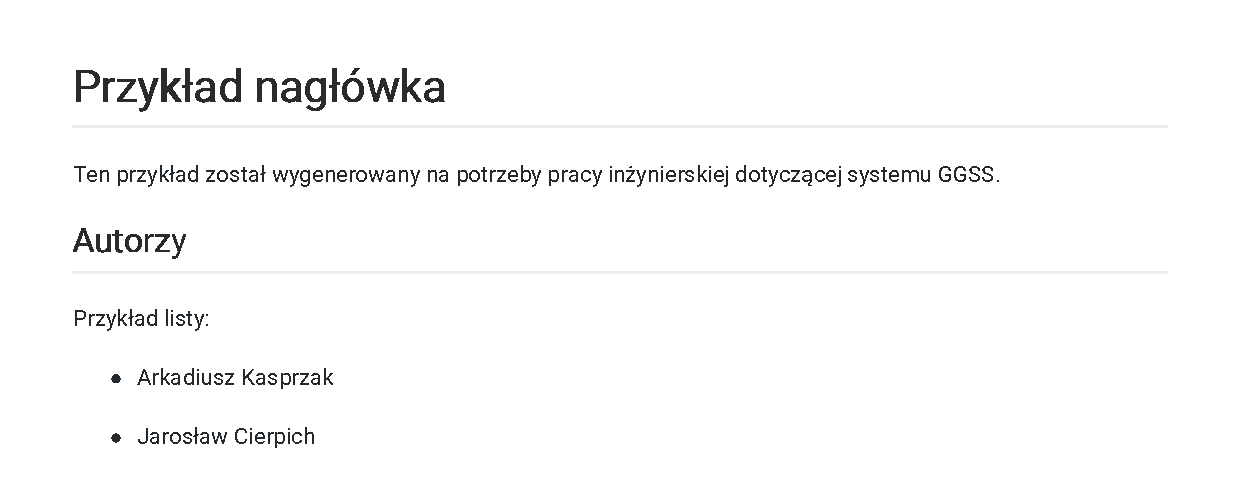
\includegraphics[width=\textwidth]{res/MarkdownExample}
\end{figure}


\subsection{Opis wykonanej dokumentacji}
Dla każdego repozytorium w projekcie wykonany został plik \textit{README.md} zawierający informacje takie jak:
\begin{itemize}
\item opis zawartości repozytorium (np. lista bibliotek wraz z krótkim ich opisem)
\item wymagania dotyczące środowiska, w którym projekt może zostać zbudowany (np. niezbędne biblioteki zewnętrzne, wersja narzędzia \textit{CMake})
\item szczegółowy opis procesu budowania projektu wraz z gotową komendą umożliwiającą jego zbudowanie 
\end{itemize}

Rys. \ref{fig:markdownHardware} przedstawia fragment zawartości wygenerowanej za pomocą pliku \textit{README.md} znajdującego się w repozytorium \textit{ggss-hardware-libs}, opisującej proces budowania bibliotek wchodzących w skład tego repozytorium. Poza listą kroków opisującą szczegółowo budowanie zestawu biblitek, instrukcja zawiera również pojedynczą komendę, użycie której wykonuje cały proces bez konieczności dodatkowego wkładu ze strony użytkownika. Takie podejście ma na celu ułatwienie osobom nieznającym struktury projektu szybkie jego zbudowanie. Podobne komendy umieszczone zostały w repozytoriach zawierających aplikacje wchodzące w skład systemu GGSS (takie jak \textit{ggssrunner}).

\begin{figure}
\centering
\caption{Fragment instrukcji budowania zestawu bibliotek znajdujących się w repozytorium \textit{ggss-hardware-libs}}
\label{fig:markdownHardware}
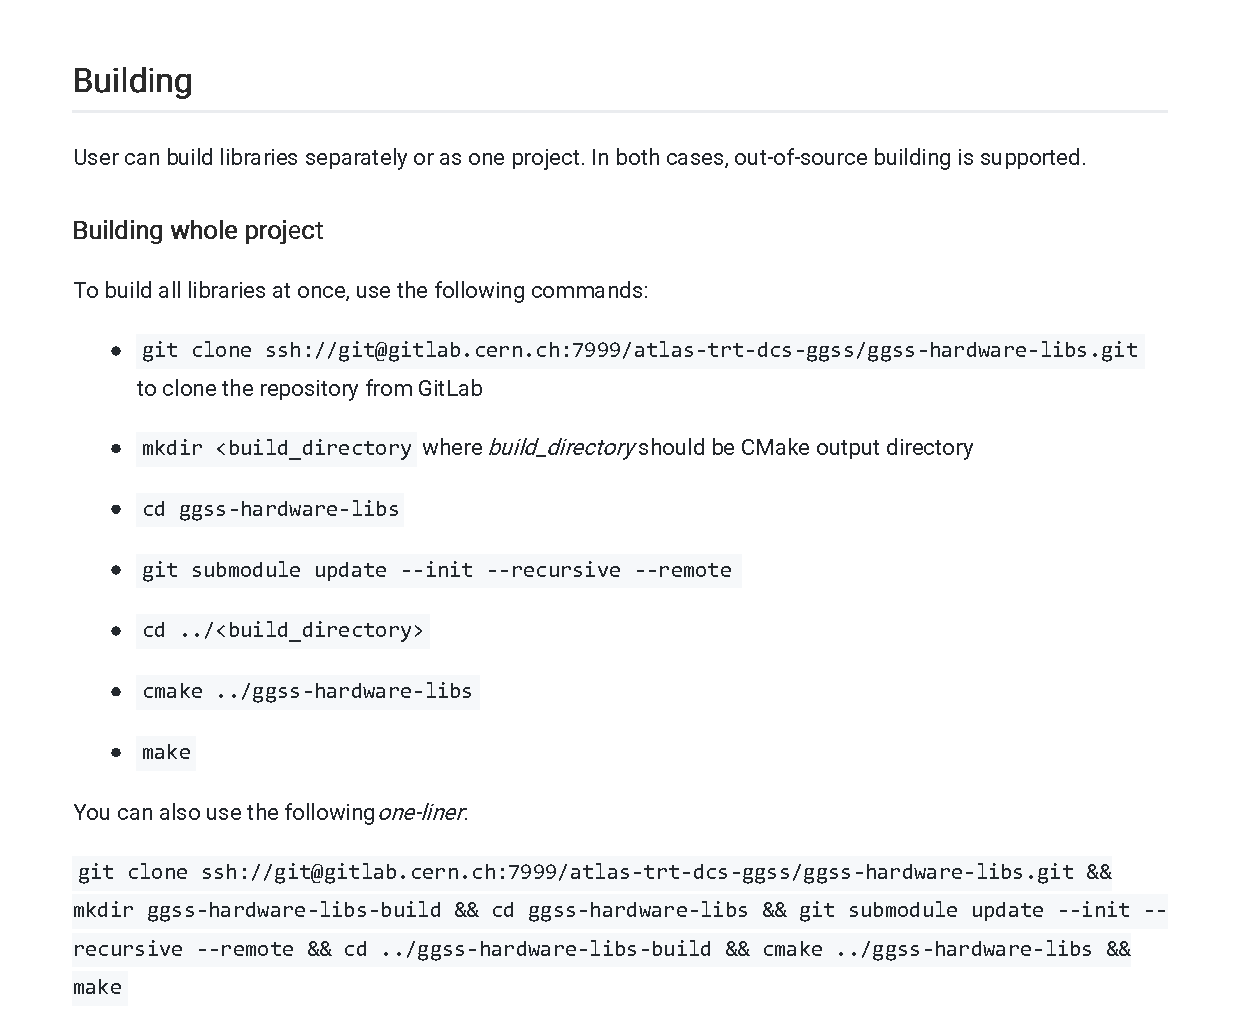
\includegraphics[width=\textwidth]{res/HardwareLibs}
\end{figure}

Oprócz plików \textit{.md} przygotowane zostały również dwa dokumenty opisujące ważne, zdaniem autorów, aspekty utrzymania i rozwoju projektu GGSS. Dokumenty te zostały dołączone do niniejszej pracy w formie dodatków (\ref{appendix:A2} oraz \ref{appendix:A3}). Dotyczą one rozszerzania projektu o nowe moduły (dodatek \ref{appendix:A2} - \textit{Adding new modules to the project using existing CMake
templates}) oraz przygotowywania maszyny wirtualnej do pracy jako \textit{runner} w procesie CI/CD (dodatek \ref{appendix:A3} - \textit{Preparing virtual machine to work as a runner}). 
